% docs/texte/20_core/sky.tex -- chapter "Sky Models" (Interferosim)
% Version: 0.2.0 (2026-10-12) -- package interferosim.sky implemented
%   0.1.0: placeholder
% ================================================================
\label{ch:sky-models}
\index{sky model}
The package \texttt{interferosim.sky} describes the sky as a field centre
plus a list of components (Fig.~\ref{fig:uml-model}). The theory of the
component visibilities is given in chapter~\ref{ch:visibility}.

\section{Components}

\begin{center}
\begin{tabular}{@{}lll>{\raggedright\arraybackslash}p{5.6cm}@{}}
\toprule
\texttt{kind} & Class & Parameters & Visibility \\
\midrule
\texttt{point} & \texttt{PointSource} & -- & $S\,e^{-2\pi i(ul_0+vm_0)}$ \\
\texttt{gauss} & \texttt{GaussianSource} & \texttt{fwhm\_x\_deg}, \texttt{fwhm\_y\_deg}, \texttt{pa\_deg}
               & elliptical Gaussian, analytic \\
\texttt{disc}  & \texttt{DiscSource} & \texttt{diameter\_deg}, \texttt{limb}, \texttt{limb\_power}
               & $2J_1(x)/x$ (uniform) or Hankel transform (limb-brightened) \\
\bottomrule
\end{tabular}
\end{center}

All components share \texttt{name}, \texttt{dx\_deg}, \texttt{dy\_deg}
(offset east/north from the field centre) and \texttt{flux\_jy}. Point and
Gaussian components, their rendering and their visibilities are taken over
unchanged from \texttt{aas6sim}~1.3.1; the disc implements the solar model
of notebook~B with the profile $I(\rho) = 1 + \mathrm{limb}\cdot
\rho^{\,\mathrm{limb\_power}}$, $\rho = r/R$. The position angle
\texttt{pa\_deg} rotates the major axis (\texttt{fwhm\_x\_deg}) from the
$+$\texttt{dx} axis towards $+$\texttt{dy}, as in \texttt{aas6sim}.

\paragraph*{Rendering.} \texttt{SkyModel.render\_map()} returns an image in
Jy per pixel. Components smaller than two pixels are put into a single
pixel, so the total flux is conserved on every grid. By default the map
is centred on the components and sized to contain all of them.

\section{File format}

Sky models are stored as JSON in the format of the AAS6 simulation sky
(\texttt{\nolinkurl{json/interfero/sim_sky.json}}); AAS6 files can be read directly,
and files written by Interferosim can be read by AAS6 as long as they
contain only \texttt{point} and \texttt{gauss} components.

\begin{lstlisting}[basicstyle=\ttfamily\footnotesize, frame=single]
{
  "_note": "free text",
  "center": {"label": "W3(OH)", "ra_deg": 36.7661, "dec_deg": 61.8742},
  "components": [
    {"name": "Maser M1", "dx_deg": 0.3, "dy_deg": 0.45, "flux_jy": 70.0,
     "kind": "point", "fwhm_x_deg": 0.0, "fwhm_y_deg": 0.0, "pa_deg": 0.0},
    {"name": "Sun", "dx_deg": 0.0, "dy_deg": 0.0, "flux_jy": 476200.0,
     "kind": "disc", "diameter_deg": 0.5667, "limb": 0.5, "limb_power": 8.0}
  ]
}
\end{lstlisting}

Example skies are in \texttt{configs/skies/}:
\begin{itemize}
  \item \texttt{aas6\_demo.json} -- demo field of \texttt{aas6sim}
        around W3(OH) (Fig.~\ref{fig:sky-demo}),
  \item \texttt{w3oh\_masers.json} -- the three OH masers alone,
  \item \texttt{sun\_21cm.json} -- the quiet Sun at 21\,cm,
        $T_b = 10^5\,\mathrm{K}$, $34'$, limb brightening $+50\,\%$.
\end{itemize}

\section{Maps}

\texttt{interferosim.plotting.plot\_sky\_map()} shows a sky model as a map
(logarithmic, linear or asinh scale, east to the left, axis unit chosen
from the field size). Components smaller than a few pixels are marked by
circles whose area is proportional to their flux density.
\texttt{plot\_sky\_overview()} adds a zoom, e.g.\ on the maser group.
Outside Jupyter the command
\begin{lstlisting}[basicstyle=\ttfamily\footnotesize]
interferosim-sky configs/skies/aas6_demo.json --overview -o demo.png
\end{lstlisting}
writes the same map to a file. The notebook
\texttt{notebooks/01\_sky\_models.ipynb} shows all examples and how to build
a sky model of one's own.

\begin{figure}[htbp]
  \centering
  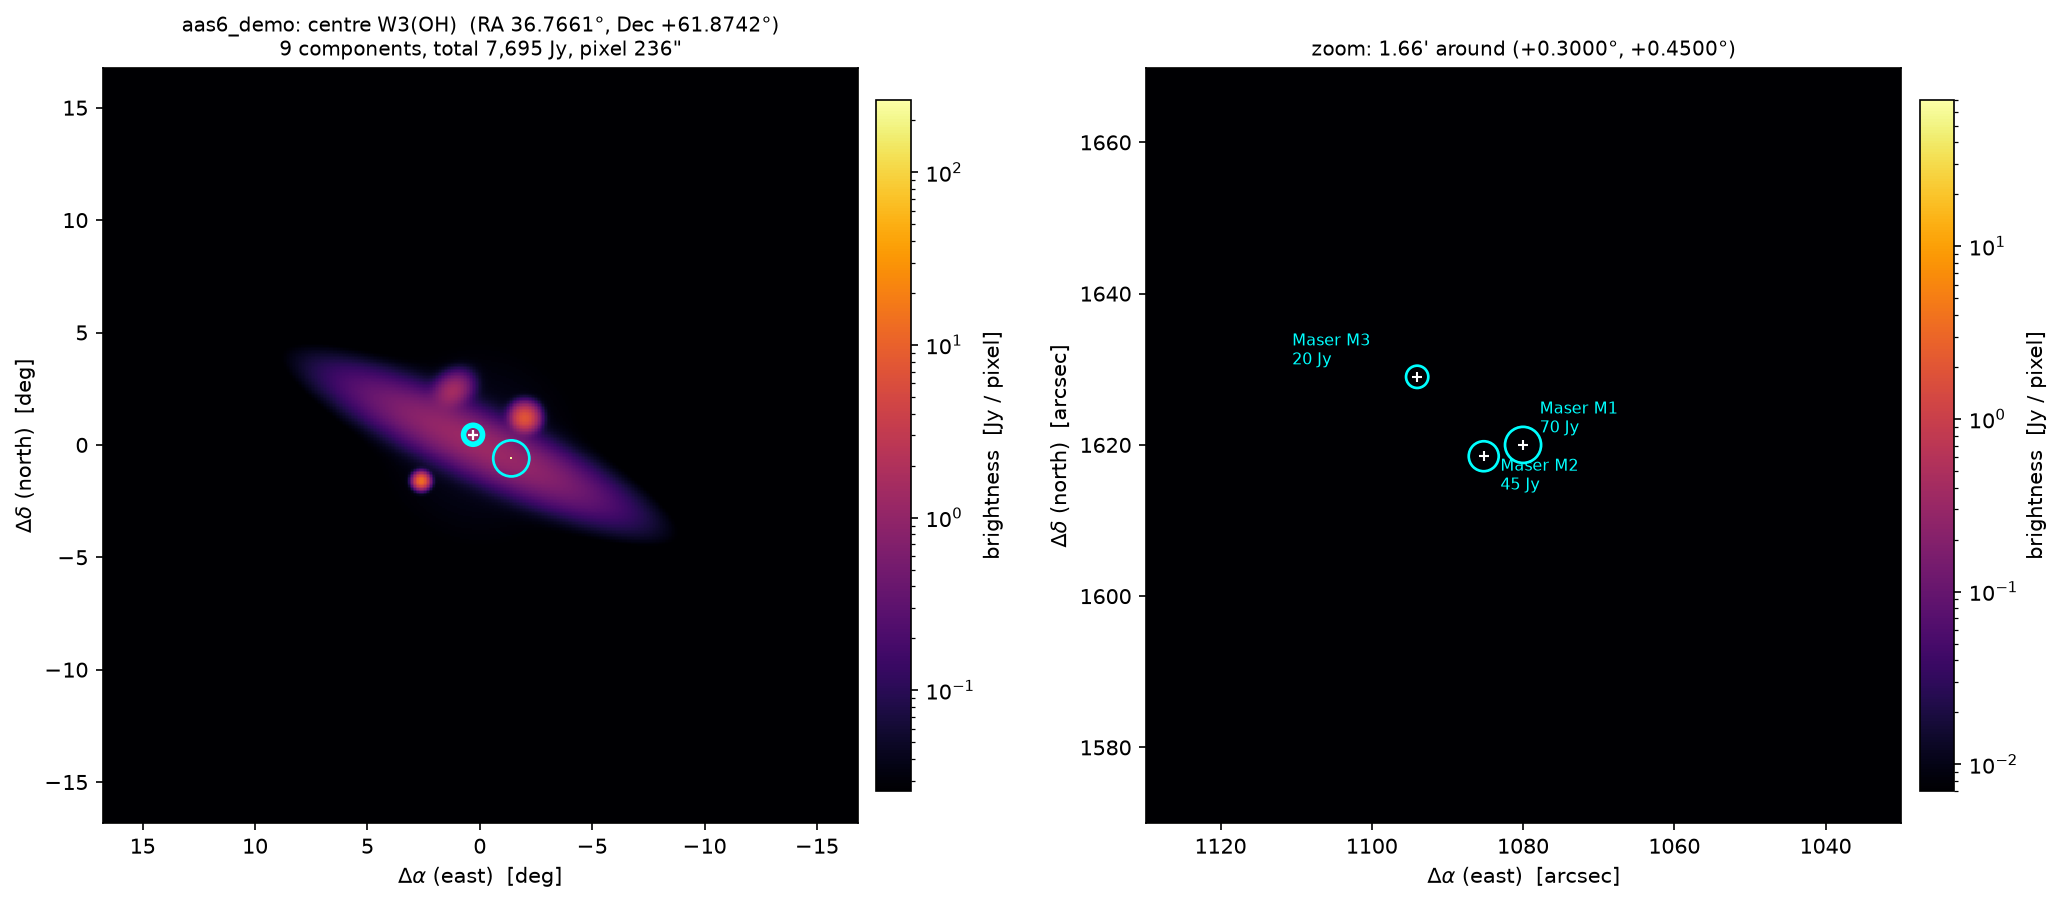
\includegraphics[width=\textwidth]{images/sky_demo_overview.png}
  \caption{Demo field \texttt{aas6\_demo.json}. Left: full field
           (logarithmic scale); right: zoom on the OH maser group, which
           is far below the pixel size of the full map.}
  \label{fig:sky-demo}
\end{figure}
